\title{Gravitational Wave Detection in Gaussian Noise using Deep Learning}
\author{
        Pascal Müller [pamuelle@student.ethz.ch] \\[4cm]
        A bachelor thesis supervised by\\[2cm]
        Prof. Lavinia Heisenberg
}

\date{\today}

\documentclass[12pt]{article}
\usepackage[utf8]{inputenc}
\usepackage{graphicx}
\usepackage{pdfpages}
\usepackage{hyperref}
\usepackage[parfill]{parskip}
\usepackage{amsmath}
\usepackage{hyperref}
\usepackage{soul}
\usepackage{multirow}

\usepackage{tikz}
\usetikzlibrary{shapes,arrows}

\usepackage{biblatex} %Imports biblatex package
\addbibresource{src/references.bib} %Import the bibliography file

\definecolor{LightGray}{gray}{0.9}

\newcommand{\hlc}[2][LightGray]{{%
    \colorlet{foo}{#1}%
    \sethlcolor{foo}\hl{#2}}%
}

\begin{document}
\maketitle

%!TEX root = ../thesis.tex

% TODO:
% 1. Improve quality.
% 2. Make sure we have a reference for everything. (e.g. add einstein paper)
% 3. Finish the "organized" part at the end.
% 4. Improve quality of Figure 1.
% 5. Maybe add that this is the basic for a project where new physics should
%    be found like e.g. NS eq. of state blabla.

\section{Introduction}
% Introduction to the general topic of GW
In 1916, Einstein predicted the existence of gravitational waves. With the first
detection of a gravitational wave\cite{PhysRevLett.116.061102}, emitted by two 
merging black holes, on September 14, 2015 his prediction was profen correct.
This detection marked the beginning
of the GW astronomy era. Up until then, it was also the last missing
 extrasolar messenger needed for full-scale multi-messenger physics.
\cite{Branchesi_2016} 

% Multi-Messenger physics: Importance of latency
Because multi-messenger physics utilizies different messengers to observe the 
same transient, it is of paramount interested to minimize the latency between 
the transient's actual occurence and its reported detection.

% Descibe the current situation: We have several detectors. The measurement is
% noisy.
When analyzing the \textit{strain} $s(t)$ measured by the detector, the
fundamental assumption is that it is made up by the GW \textit{signal} $h(t)$
and \textit{noise} $n(t)$ whereas

\begin{equation}
  s(t) = n(t) + h(t)
\end{equation}

Analyzing $s(t)$ about the possibile occurence of $h(t)$ is currently done by
using an approach called matched filtering. Matched filtering works by 
convoluting precalculated
models of expected signals, so called templates, with the measured data.
Because the parameters of the expected signals are not known in advance, the
template bank spans a large astronomical parameter space. This leads to
matched filtering approaches being very computationally expensive which leads
to a high latency between the occurence of the GW signal and the reported
detection. It is therefor of interest to find methods which are less
computationally expensive and thus provide a low-latency detection algorithm.


In \autoref{fig:1_data_processing}, taken from \cite{2020CQGra..37e5002A},
we can see a simplified schematic summarizing the main steps in LIGO-Virgo data
processing.  It starts with the measurement done by the detector. The
measurement undergoes a quality control to make sure the measurement is actually
useful. Once a sufficient quality has been established, the data is being
searched for GW signals and in case a signal is found (called an event),
the mergers parameters are being estimated. Each event gets a statistical
significance assigned, which is usually given by the false-alarm rate (FAR)
of the search at a ranking statistic threshold associated with the candidate 
event. The FAR is basically telling us how many false positives occured over
the duration of the analyzed data. Current low-latency searches do not distribute
any event candidates with a FAR greated than 1 per month.



% OKAY

% I now want to establish the FAP vs. FAR issue.

%Because a detector has to be upgraded and maintained it can't run all the time.
%This together with the quality control leads to the data stream being split up
%into segments. Each segment is several days to several weeks long. When
%searching for signals or trying to estimate parameters, we can't directly pass
%a whole segment. This is because a segment usually contains too much data at
%once but also because different segments have different durations. This issue is
%solved by using a sliding window of fixed duration, e.g. 1 second, and a stride
%of fixed
%duration, e.g. 0.1 second. The window is then being moved through the segment
%using the stride. E.g. a segment of 10 seconds would results in 90 one second
%mini-segments. Each such mini-segment is then passed to the needed algorithm.
%The algorithm gives a result about this 1 second of data. E.g. it might tell us
%that this 1 second of data contains a (a art of) a signal. This is called a
%trigger.
%
%The above approach of using a sliding window to feed the data to an algorithm
%leads to several sliding window giving a trigger for the same GW
%signal. Because we only want one positive alarm per GW signal, we cluster
%together close triggers.


% Describe what previous work did.

% Say what's wrong with previous work

% Make a conclusion: FAP vs FAR


Pioneering works by XX and XX showed that convolutional neural network can
distinguish between a sample containing only pure noise and noise injected
with a signal from BBH. Those works both used a similar setting. They used either
simulated gaussian or real LIGO noise and injected simulated signals into it.
Each such sample was 1s long. They used those samples to train their CNN but
also as their test set. To evaluate their network, they used the commonly used
true ositive rate and the false positive rate and computed a ROC curve using
false alarm probability. As [29] showed, this is an issue because the actual
data of a detector is continuous stream of data. False alarm probability is a
way better way to compare a deep learning algorithm to a matched filter
algorithm.

The networks tested in these works were able to distinguish
data containing a GW signal from pure noise with a false alarm probability (FAP)
of $10^{-3}$ i.e. the networks classified about 1 in 1000 pure noise samples
falsly as containing a signal.

In [29] it was shown that this approach (FAPs) does not directly translate to
false alarm rates (FARs) on continous data streams. The appropriate question to
asl is: How many false signals does the network identify per time interval of
continous data, as opposed to how many uncorrelated data chunks are falsely
identified as containing a signal. Furthermore, comparing deep learning to
matched filtering is hard because the later works on way lower FARs.


In this thesis,
we will explore a similar deep learning (DL) approach to search for simulated GW
signals in simulated Gaussian noise. While training a neural network (NN) is also
rather computationally expensive, the evaulation of a trained NN can be done in
a fraction of a second. Furthermore future detections can easily be incorporated
leading to an improved neural network.

TODO: Because this work might become the fundation for a bigger project and
because it was approached in a very open way, the code is rather general and
easily extendable to a more general case.

This thesis is organized as follows. In Section 2 we first establish the data
used for our DL approach. In section 3 we will describe the actual DL approach.
In section 4, we present the results. In section 5 we discuss possibilities for 
future work.

\begin{figure}
  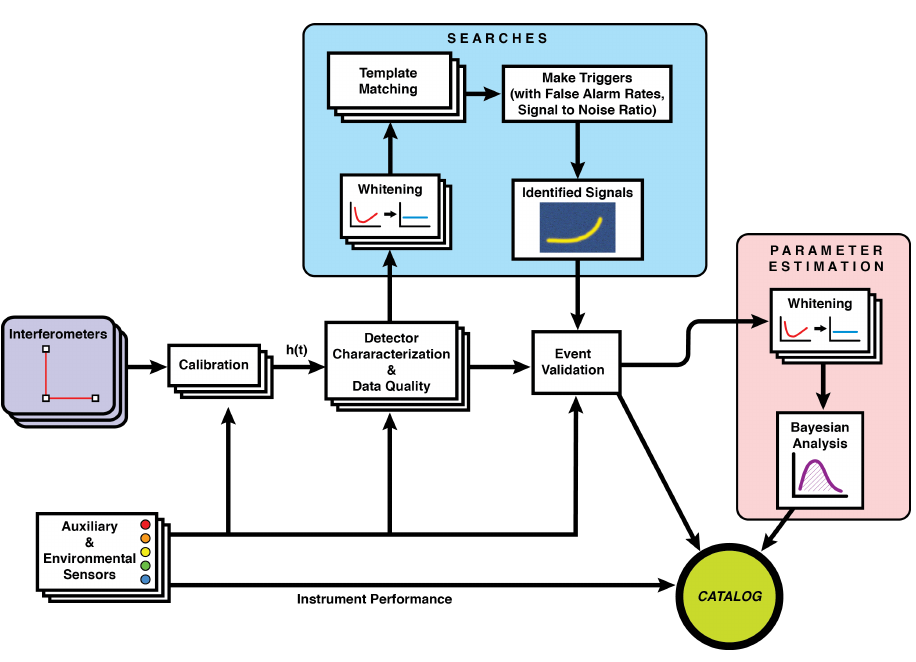
\includegraphics[width=\textwidth]{img/1_introduction/data_processing.png}
  \caption{asd}
  \label{fig:1_data_processing}
  \centering
\end{figure}




%!TEX root = ../thesis.tex

\section{Data Generation}
% Give quick intro into what kind of data is needed for a DL approach.
In deep learning, one basically tries to fit a mathematical model, the neural
network, to a data set consisting of measurements. This process is called
\textit{learning}.
Those measurements might be data from a physical experiment, time series from
the stock market, health information collected for mice or virtually and
other source of data.

In most cases, the data is split into three sets. The first subset is used to
train the neural network and is called \textit{training set}. The second subset 
is used to validate the learning progress and is called \textit{validation set}.
This process of learning and validating is repeated until we think the trained
NN can make good predictions. In a last step we use the trained NN to make an
unbiased prediction on the third subset, called \textit{test set}.

In the case of GW we only have a very limited data set of measurements. We can't
make an experiment to easily generate more measurements, we can only try to 
detect the ones which occure naturally. This rises the problem of needing to 
know how a gravitational wave looks like to be able to measure it. We solve this
by simulating GW waveforms and injecting it into Gaussian noise.

\subsection{Training and Validation Set}
% Parameters for signal
To generate the training and validation set, we first generate 200'000 signal
waveforms sampled at 2048 Hz with a duration on average of around several seconds.
This is done by drawing the following parameters for each waveform.
We use the \hlc{SEOBNRv4\_opt} approximant. The
two masses $m_1, m_2$ are drawn uniformly between $10 \textup{M}_\odot$ and
$50 \textup{M}_\odot$ whereas $m_1 < m_2$. The coalescence phase, inclination and
polar angle are also drawn uniformly between $0$ and $2 \pi$. Furthermore we use
\hlc{self.sky\_location\_dist.rvs()[0]} to compute the declination and right
ascention. We also use a low frequency cutoff of 18 Hz.

Each such waveform has a duration of several section i.e. they are not the same.
We stated before, that we want to use 1 second i.e. not the full waveform. A
 waveform consists of three parts: The inspiral part, the actual merger and the
 ring down part. Since we want 1 second but have several seconds, the question
 arises, which part of the waveform we take.

 What we do is we cut 1.25 seconds around the merger. Doing so would lead to
 all samples having the merger at the same place: in the middle. To make sure
 our NN doesn't learn such information, we place the merger randomly inside this
 1.25s window by 0.2 seconds. This will add stability to our NN. We end up with
 a 1.25s long sample containing the merger. We use 1.25seconds because of post
 processing.

% Parameters for noise
Next we generate 400'00' pure gaussian noise samples, again sampled at 2048 Hz.
The noise is generated using the \hlc{pycbc.psd.aLIGOZeroDetHighPower}
PSD with
a low frequency cutoff of 18 Hz. Note that to compute the value for the
frequency delta, we use a duration of 1.25s. Because we can generate noise for
a chosen length, we don't have to do any post processing like we did with the
signals


% Generating samples
At last we need to generate the actual samples used to train and validate the NN
. This is done by injection all 200'000 signal samples into 200'000 of the
400'000 noise samples. From [ml strategies] we see that the best training is
done on samples with SNR of 8. This is because low SNR signals generalize while
high SNR don't. Because of this, we rescale all signals to an SNR of 8. We then
inject it into one of the noise samples. Once the injection is done, we whiten
the whole sample. Whitening it reduces the duration from 1.25s to 1s. This is
because the edges get corrupted because the math assumes infinity blabla. The
remaining 200'000 pure noise samples are also whitened.

We end up with 400'000 samples of 1 seconds whereas half of it contains a signal
and the other half doesn't. We call them \textit{pure noise} and 
\textit{noise + signal}.

TODO: Explain whitening

\subsubsection{Implementation}
Explain implementation

\subsection{Test Set}
The test set consists of 1 month of data. In this work, we use the ml challenge
generation script with the first dataset. It has some properties yada yada yada.

I used MLGWSC for it because there are several sets and it gave the possibility
of making it more general. 

\subsubsection{Implementation}
Explain implementation


%!TEX root = ../thesis.tex

\section{Deep Learning Approach}
% Introduction: High-level overview about general idea behind DL.
% Main Workflow: Describe the main workflow (train + eval in each epoch)
% Training: Describe training
% Evaluation: Describe evaulation (incl. accuracy and efficiency)

% Quick introduction to deep learning
Deep learning is a machine learning approach which consists of processing
units, so called neurons, which are arranged in an array. Such an array makes up
a layer. One to several such layers make up a neural network (NN). Each neuron
acts like a filter extracting higher-level features from the raw input. On a 
basic level, a neural network is trained by repeatedly applying the training
data and comparing its results with the known labels.

% Extend on the introduction
For the DL approach one needs a training set and a test set. The training set
is split whereas 80\% is used for the actual trianing of the NN and 20\% is used
to evaluate the trained NN in each epoch. 

% Provide pseudo code for main workflow
As we can see in pseudocode X, we havet his workflow. yada yada yada

% Provide pseudo code for train()

% Provide pseudo code for validation()



In this thesis the neural network from \cite{schaefer2021training} is used.
TODO: FAR like used in gabbart et al is "wrong", so use ml strategies approach.




%!TEX root = ../thesis.tex

\section{Results}
In \autoref{fig:4_losses} we can see the evolution of training and validation
loss during a 200 epochs run. In this run, the NN as described in chapter 3 and
the training data as described in chapter 2 was used. The NN converges fast
until about epoch 60. After epoch 60 training and validation loss start to
slowly diverge, indicating that the NN started to overfit on the training data.
Apparently it even converges a little bit faster than the corresponding 
experiment in \cite{PhysRevD.105.043002}.
\footnote{According to Ondřej Zelenka in a private discssion on Slack on
  24.01.22} I accord this to the difference in training set. The state of the
NN at epoch 59 was chosen as the \hlc{best\_weights.pt}.

\begin{figure}[ht]
  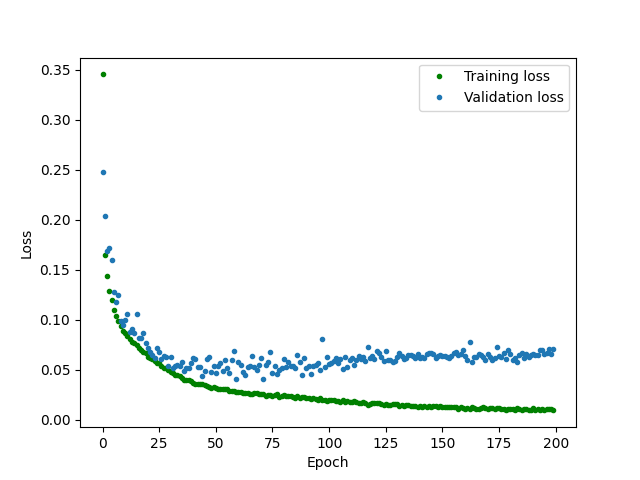
\includegraphics[width=\textwidth]{img/4_results/losses.png}
  \caption{Training and validation loss over 200 epochs.}
  \label{fig:4_losses}
  \centering
\end{figure}

In \autoref{fig:4_eff} we can see how the efficiency evolved over the 200 epochs.
Again we have a fast improvement of the efficiency and after about epoch 40 it
converged to about 0.9, which is similar to what the authors of
\cite{PhysRevD.105.043002} observed.

\begin{figure}[ht]
  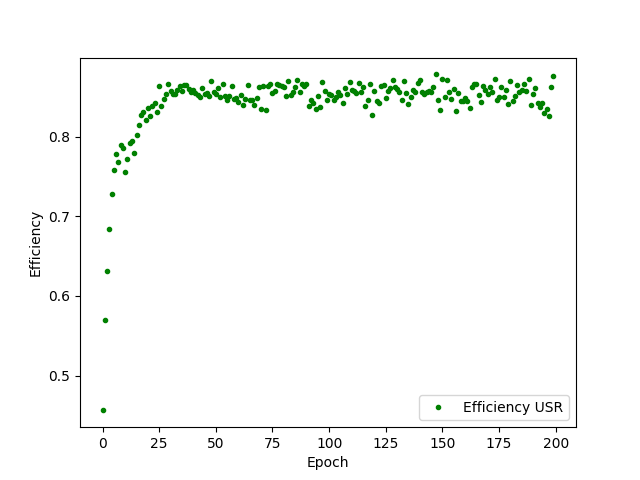
\includegraphics[width=\textwidth]{img/4_results/efficiencies.png}
  \caption{eff.}
  \label{fig:4_eff}
  \centering
\end{figure}

The low loss as well as the high efficiency are good indicators for a good
performance of our NN. To evaluate how good the NN actually is, two numerical
experiments were made. The first one was applying the network to a small test
set with short duration. The second one was applying the neural network to test
data of 1 month and computing a sensitivity plot.

\subsection{Experiment 1: Short Test Data}
In this experiment, a short strain of noise was generated and injected with 5
signals at different SNR. The whole strain was whitened and analyzed by the
neural network.

In \autoref{fig:4_apply_single} we can see a plot consisting of three windows.
The top window displays pure noise in blue with the 5 signals overlayed. Note
that it does in the top window, the signals are not yet injected into the noise.
In the middle window, we can see the whitened noise+signal strain. In the bottom
window, the p-score of the network is plotted.

As we can see, the network detects all signals and assigns a pscore of 1 for all
of them but it sometimes also assigns a high pscore value to noise. Noteworthy
is also the difference between the thickness of the bars in the bottom window.
The bars indicating signals are thicker because we use a sliding window to feed
the data to our NN, leading to several windows containing the same merger.

The result to this experiment made me confident, that the NN does indeed
recognize GW signals injected in whitened Gaussian noise.

\begin{figure}[ht]
  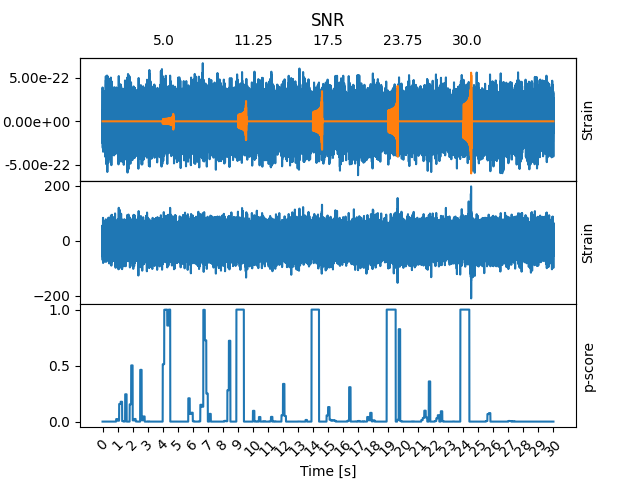
\includegraphics[width=\textwidth]{img/4_results/apply_single.png}
  \caption{apply single.}
  \label{fig:4_apply_single}
  \centering
\end{figure}

\subsection{Experiment 2: 1 Month of Test Data}
In this experiment, we analyze a month of test data, compute the FAR as well as
the sensitive distance and plot it. Computing the FAR as well as the
sensitivity distance is done with code prodived by \cite{MLGWSC1}.

\begin{figure}[ht]
  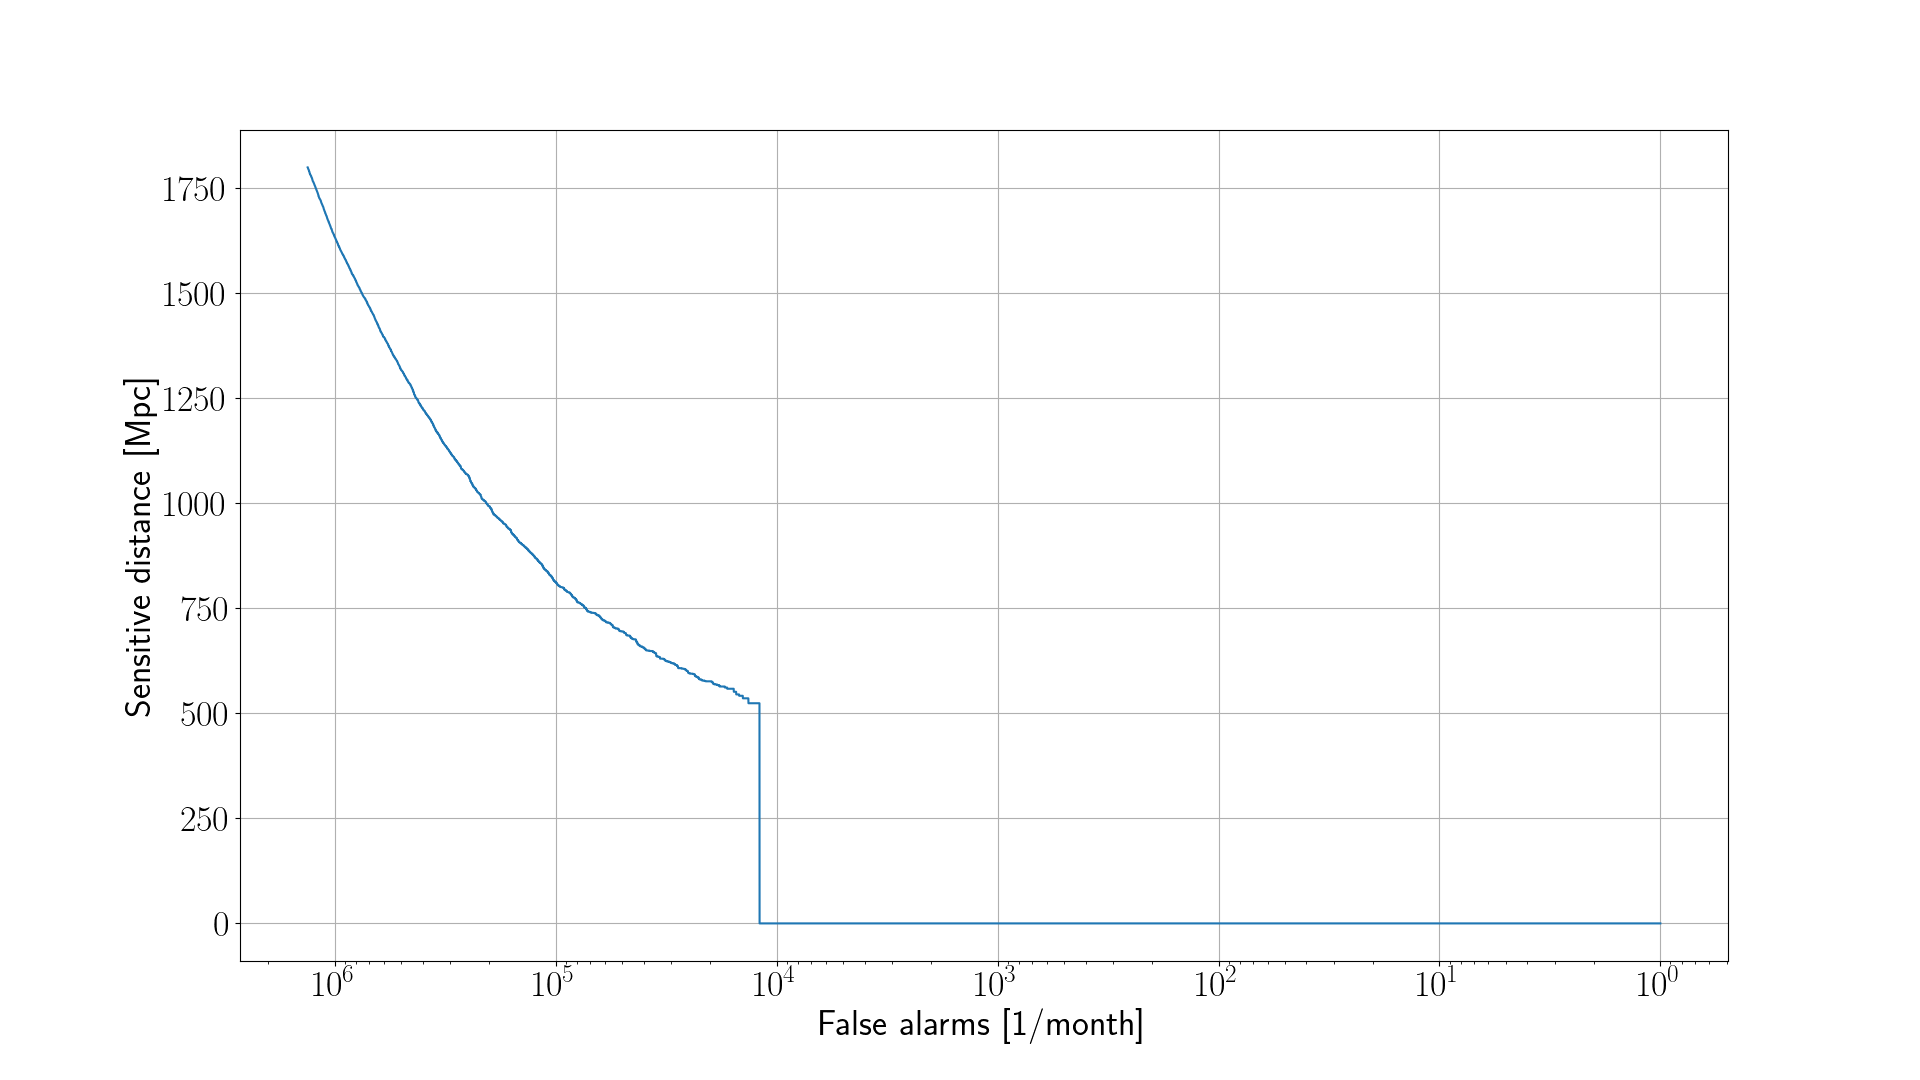
\includegraphics[width=\textwidth]{img/4_results/sensitivity_plot.png}
  \caption{The NN applied to short test data.}
  \label{fig:4_sensitivity_plot}
  \centering
\end{figure}

The plot indicates how many false alarms per month are found. For mergers which
are further away and thus are generally harder to measure we can expect a higher
number of false alarms. In the plot we can see this behaviour. Furthermore note
the sudden drop in sensitivity distance around $10^4$ false alarms. This is
because for this plot, the softmax output layer was used. If the USR output
layer would have been used, we would see a smooth continuation of the graph. The
reason this isn't included is because the corresponding data got lost in an
technical accident and reapplying the network would have taken too long on my
limited hardware.

While this plot seems to indicate a successfull analysis of test data, I think
it actually shows the opposite. In \hlc{MLGWSC/mock/ds1.ini} we can see that
we used a maximal
chirp distance of $350$ mpc. Because of this, I'd expect the maximal
sensitivity distance to be of around 6'000 and not 1750.

Despite this result, I'm still confident that the network itself works. This is
because of the first experiment. I think the issue that led to this bad result
can be found in the data pipeline used to split up the 1 month of data but in
the end, that's just a guess.

My conclusion is nevertheless positive. I was able to find GW signals injected
in Gaussian noise and got to explore the space of GW analysis using ML methods
in depth which presented itself as a challenging but instructive experience.

This thesis is hosted on
\url{https://github.com/pascal-mueller/bachelor_thesis}

%%!TEX root = ../thesis.tex

\section{Future Works}


\section{Acknowledgements}

I want to thank Prof. Lavinia Heisenberg for supervising me on this thesis and 
Prof. Steven Schramm from the University of Geneva for his consultation. I also
want to thank Ondřej Zelenka from Friedrich-Schiller-Universität Jena and Marlin
Schäfer from Leibniz Universität Hannover for their help in understanding their
work. I also want to thank everyone for all the discussions we had.

\newpage

% References
\printbibliography %Prints bibliography

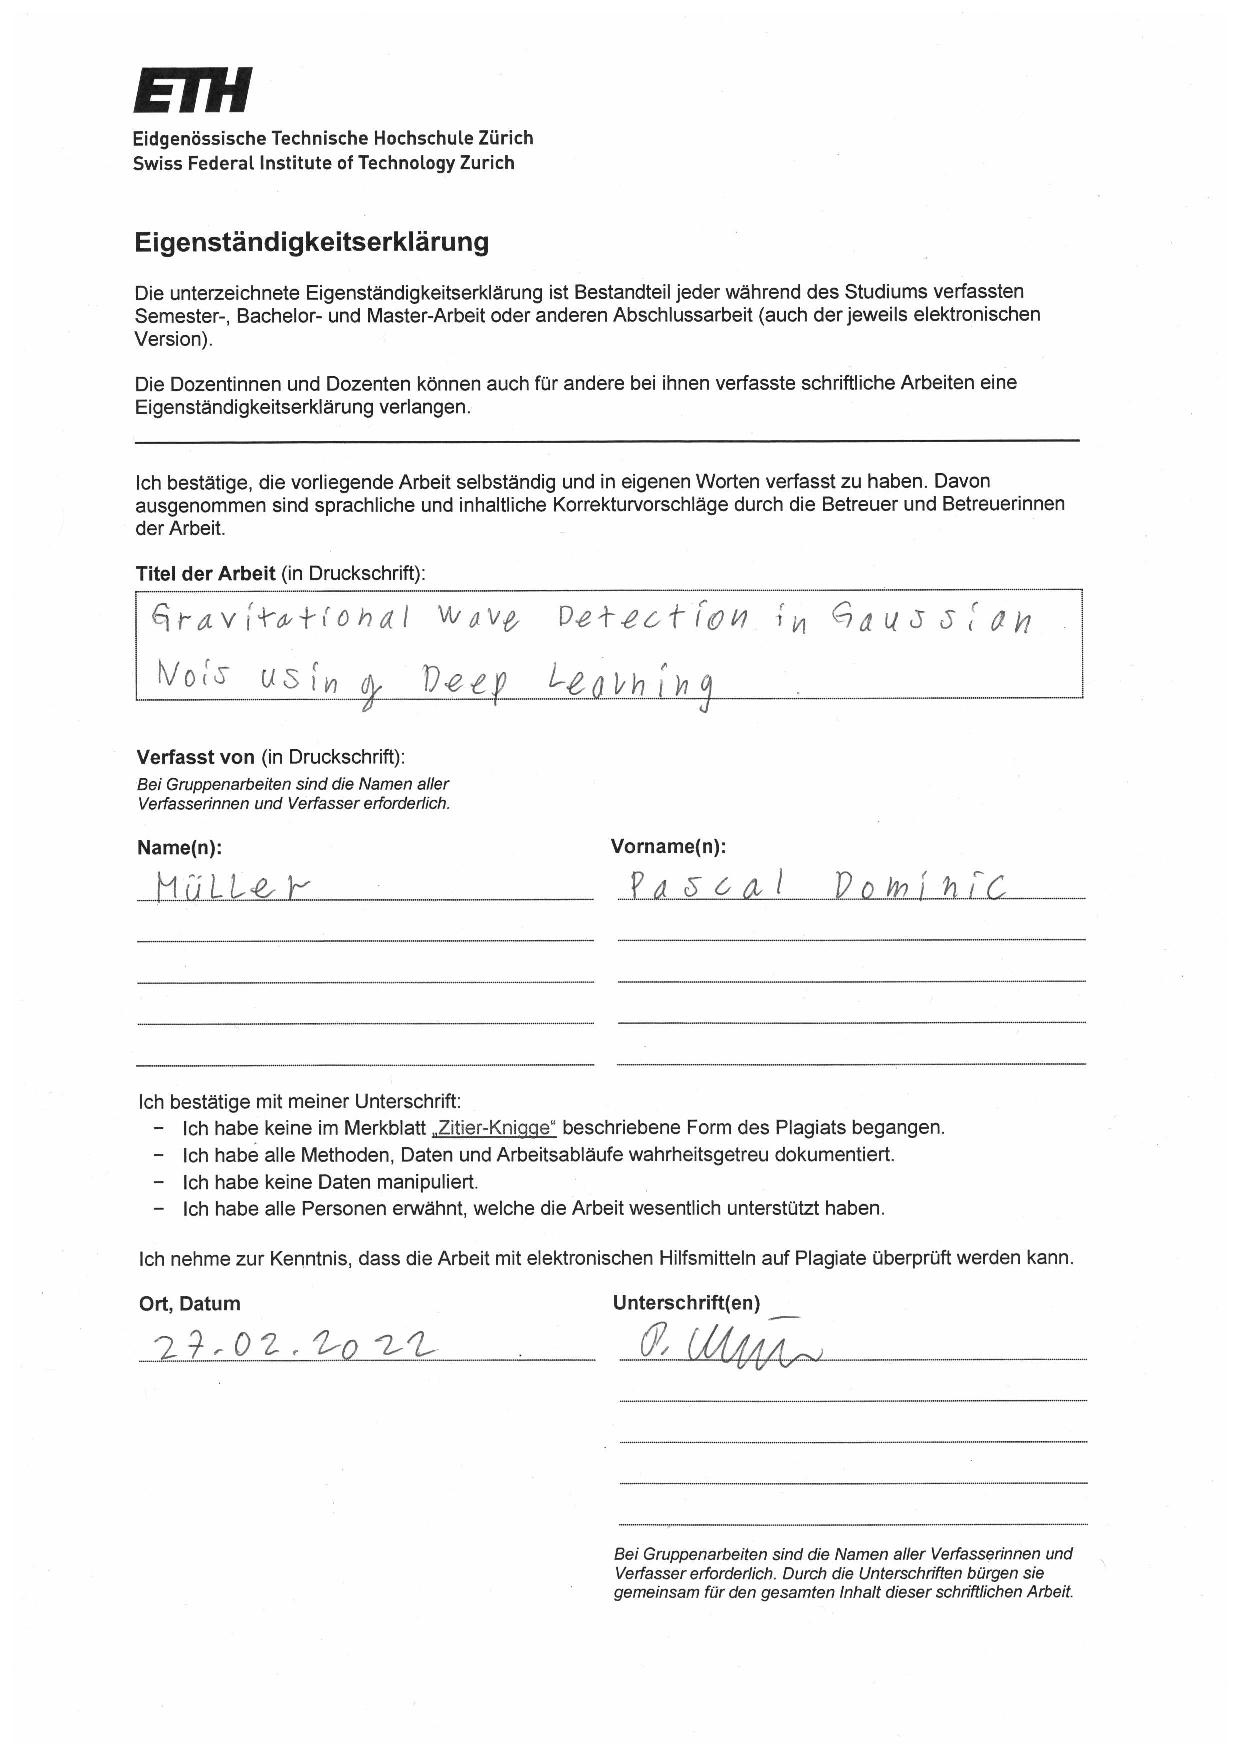
\includepdf[pages={1}]{erk.pdf}

\end{document}
